\section{Claim formalization annotation}
\label{sec:formalization_annotation}

\subsection*{Cheat sheet}

\textbf{Task}: Transform natural language claims into logical form. Logical form needs to have:
\begin{itemize}
\item Domain individuals 
\item Claim relation
\item Type
\item (Opinion holder)
\end{itemize}

\vspace{0.3cm}

\noindent \textbf{Domain individual} \\
Find appropriate individuals mentioned in the claim (i.e. \textit{marijuana consumers},
\textit{brain damage}, \textit{legalized tobacco}, \textit{heroin}, \textit{mafia selling marijuana}) \\

\pagebreak

\noindent \textbf{Claim relations} \\

\begin{table}[h!]
\begin{tabular}{| l |  p{9cm} | p{3cm}| }
\hline
\textbf{Promotes} & 
\makecell[cc]{
\texttt{has\_antecedent + domain\_individual} \\
\texttt{promotes + domain\_individual}
}
& 
fosters, brings about, leads, forces, advances \\
\hline
\textbf{Implies} &
\makecell[cc]{
\texttt{has\_antecedent + domain\_individual} \\
\texttt{implies + domain\_individual}
}
&
if .. then .. is \\
\hline
\textbf{Causes} & 
\makecell[cc]{
\texttt{has\_antecedent + domain\_individual} \\
\texttt{causes + domain\_individual}
}
& causes \\
\hline
\textbf{Suppresses} & 
\makecell[cc]{
\texttt{has\_antecedent + domain\_individual} \\
\texttt{suppresses + domain\_individual}
} &
inhibits, stops, decreases \\
\hline
\textbf{Contradicts} & 
\makecell[cc]{
\texttt{has\_antecedent + domain\_individual} \\
\texttt{contradicts + domain\_individual}
} &
if .. then not .., is .. not a \\
\hline
\textbf{Does not cause} &
\makecell[cc]{
\texttt{has\_antecedent + domain\_individual} \\
\texttt{does\_not\_cause + domain\_individual}
} &
causes not, does not cause \\
\hline
\textbf{Declaration} &
\makecell[cc]{
\texttt{has\_declaration + domain\_individual}
} &
defines, exists \\
\hline
\textbf{Comparison} &
\makecell[cc]{
\texttt{comparison\_greater + domain\_individual} \\
\texttt{comparison\_less + domain\_individual} \\
	(\texttt{comparison\_property + domain\_individual})
} &
less than, more than, greater than \\
\bottomrule
\end{tabular}
\end{table}

\noindent \textbf{Type} $\Rightarrow$ \texttt{has\_type + fact/good\_value/bad\_value/policy} \\

\noindent \textbf{Opinion holder} $\Rightarrow$ \texttt{has\_opinion\_holder + domain\_individual} \\

\subsection*{Examples cheat sheet}

\noindent \textbf{Promotes} \\
\begin{tabular}{p{8cm} p{8cm}}
Marijuana legalization increases crime rates. & \texttt{legalized\_marijuana promotes crime} \\
Smoking marijuana makes people happy. & \texttt{marijuana\_consumer promotes happiness}
\end{tabular}

\noindent \textbf{Implies} \\
\begin{table}[h!]
\begin{tabular}{p{8cm} p{8cm}}
Marijuana is a drug. & \texttt{marijuana implies any\_drug} \\
	If we legalize marijuana, the government will earn money.  &\texttt{legalized\_marijuana implies government\_making\_money}
\end{tabular}
\end{table}
 
\noindent \textbf{Causes} \\
\begin{tabular}{p{8cm} p{8cm}}
	Marijuana consumption causes death. & \texttt{marijuana\_consumer causes death}  \\
	Marijuana legalization made government each money. & \texttt{legalized\_marijuana causes government\_earning\_money}\\
	Marijuana use alters the mind. & \texttt{marijuana\_consumer causes mind\_influential. }
\end{tabular}

\noindent \textbf{Suppresses}  \\
\begin{tabular}{p{8cm} p{8cm}}
	Legalizing marijuana hurts the balance of the economy. & \texttt{legalized\_marijuana suppresses government\_making\_money} \\
	Consuming marijuana decreases aggressive behavior. & \texttt{marijuana\_consumer suppresses aggressive\_behavior} \\
	Legalizing marijuana lowers the number of consumers. & \texttt{legalized\_marijuana suppresses marijuana\_consumer}
\end{tabular}

\noindent \textbf{Contradicts} --- be careful with double negation! \\
\begin{tabular}{p{8cm} p{8cm}}
	If legalization of marijuana happens, there will be no crime. & \texttt{legalized\_marijuana contradicts crime} \\
	Tobacco is not a plant. & \texttt{tobacco contradicts any\_plant}
\end{tabular}

\noindent \textbf{Does not cause} --- be careful with double negation! \\
\begin{tabular}{p{8cm} p{8cm}}
	Consuming marijuana does not cause death. & \texttt{marijuana\_consumer does\_not\_cause death} \\
	Legalizing marijuana never helped the government economy. & \texttt{legalized\_marijuana does\_not\_cause government\_making\_money}
\end{tabular}

\noindent \textbf{Declaration} \\
\begin{tabular}{p{8cm} p{8cm}}
	Marijuana is widely used. & \texttt{declaration marijuana\_consumer}  \\
	Marijuana should not be legalized. & \texttt{declaration illegal\_marijuana} \\
	I don’t consume marijuana.  & \texttt{declaration non\_marijuana\_consumer}
\end{tabular}

\noindent \textbf{Comparison} \\
\begin{tabular}{p{8cm} p{8cm}}
	Alcohol is more stimulative than marijuana. & \texttt{comparison\_more alcohol + comparison\_less marijuana + comparison\_property stimulative\_behavior}\\
	Heroin is worse than marijuana. & \texttt{comparison\_more heroin + comparison\_less marijuana}
\end{tabular}

\subsection*{Introduction}

The goal is to transform natural language claims to logical form given claims
and rules for annotation of logical form. This document explains the rules for
annotation. For example, given a claim ``The government will make a huge profit
from legalizing marijuana'' made on the topic of \textit{Drug legalization} by an author
named \textit{Fred}, we wish to transform it into logical form which would be: \\

\noindent \texttt{
author(Fred) $\wedge$ has\_claim(Fred, c) $\wedge$ has\_type(c, fact) 
$\wedge$ has\_antecedent(c, marijuana\_legalization) 
$\wedge$ implies(c, government\_profit)
} \\

\noindent The logical form and its rules are defined by the ontology that has been
pre-created for each topic. To annotate data, you will need to use a tool named
\textit{Protege} to load the ontology. 
The outline of the annotation is: 
\begin{enumerate}
\item Open Protege and load pre-created ontology
\item Read and understand the claim individual and its entire post.  
\item Transform the claim individual to logical form in Protege by adding properties to the claim
individual. 
\end{enumerate}

\subsubsection*{Setup}

To annotate data you will need:
\begin{enumerate}
\item Download and install Protege 5, an ontology tool
\item Load provided ontology in Protege 5
\end{enumerate}
Download and install the desktop version of Protege 5. Links for Windows instructions:
\begin{itemize}
\item \url{https://protege.stanford.edu/products.php#desktop-protege}
\item \url{https://protegewiki.stanford.edu/wiki/Instal_Protege5_Win}.
\end{itemize}

\subsection*{Annotation steps}

All the annotation will be done in the individuals tab of Protege. 
We discern between \textbf{domain} and \textbf{claim individuals}. 
\textbf{Domain individuals} are domain-specific as they
were mentioned previously in the debate, \textbf{claim individuals} are individuals
representing the logical form of natural language claims. 
You need to formalize natural language claims 
by recognizing claim relation and domain individuals
used to add properties to a \textbf{claim individual}. In total, you need to do \textbf{four}
steps to annotate a natural language claim:
\begin{enumerate}[label=\textbf{Step \arabic*.}, leftmargin=2cm]
\item select which domain individuals from a predefined list are used in the claim,
\item recognize which claim relation is used in the claim individual, 
\item which type was used for the claim (\texttt{fact/value/policy}), and 
\item identify the claim opinion holder. 
\end{enumerate}


\subsubsection*{Step 1: Choosing domain individuals}

We offer a list of \textbf{domain individuals} to choose from beforehand (loaded with
the ontology). We consider domain individuals well-established topics in the
debate as the authors mostly agree on them. Examples are: \textit{mafia selling
marijuana, marijuana tax, marijuana legalization, alcohol, science, obesity} \dots
They are usually nouns with adverbs. Some domain individuals are very similar
and it’s important to find the appropriate, most specific one, since you will
be offered both \textit{marijuana} and \textit{legalized marijuana}, you need to recognize which
domain individual is most appropriate given the claim. In case you don’t see an
appropriate domain individual, add a comment to the claim. We expect this to be
the case in ~15\% of the time. The goal of using domain individuals is to
transform sentences into logical with a minimal loss in meaning. Sometimes, you
will need to transform sentences from active to passive, or make verb nouns. 
For example, even though \textit{marijuana legalization}, \textit{marijuana legalizing} and
\textit{legalized marijuana} are three different concepts, we consider them the \underline{same
domain individual}. 

\subsubsection*{Step 2.2: Recognizing claim relations}

Claim relations are usually, but not always, indicated by the main verb or the
conjunction in the claim. We’ve noticed four basic different claim relations
with four more sub relations (we highlight sub relations in the table with
$\rightarrow$). In the table below, we list the claim relations, possible
indicators that might hint the claim relation, the pattern in which the claim
relation might appear in natural language with respect to domain individuals
(A, B, C represent any domain individual) and an example of a natural language
claim containing the claim relation. 

\begin{table}[h!]
\begin{tabular}{| l | p{3.5cm} | p{3cm} | p{5cm}| }
\hline
\cellcolor{gray!25} Claim relation & \cellcolor{gray!25}Indicators &
\cellcolor{gray!25} Pattern & \cellcolor{gray!25}Example \\
\hline
	\textbf{Promotes} & 
	Promotes, fosters, brings about, leads, forces, advances & 
	\textbf{A} promotes \textbf{B} &
\textit{Marijuana legalization improves health} \\
\hline
	$\rightarrow$ \textbf{Implies} & 
	Implies, entails, if \dots then, is &
	\textbf{A} implies \textbf{B} &
\textit{If marijuana is legal, the crime rate will rise. } \\
\hline
	$\rightarrow$ \textbf{Causes} &
	Causes &
	\textbf{A} causes \textbf{B} &
\textit{Marijuana legalization causes an increase in crime rate.} \\
\hline
	\textbf{Suppresses} &
	Similar to promotes, but negative inhibitor &
	\textbf{A} suppresses \textbf{B} &
	\textit{ Marijuana hurts health. } \\
	\hline
	$\rightarrow$ \textbf{Contradicts} &
	Does not imply, if \dots then not, is not &
	\textbf{A} implies not \textbf{B} &
\textit{If marijuana is legal, no crime will happen. } \\
\hline
	$\rightarrow$ \textbf{Does not cause} &
	Does not cause &
	\textbf{A} does not cause \textbf{B} &
\textit{Growing marijuana at home does not stop mafia selling marijuana. } \\
\hline
	\textbf{Declaration} &
	defines, exists &
	\textbf{A} &
\textit{Legalized marijuana exists.} \\
\hline
	\textbf{Comparison} & 
	Is more than, has more, does less &
	\textbf{A} is more than \textbf{B} by criteria \textbf{C} &
\textit{Marijuana is less addictive than alcohol} \\
\hline
\end{tabular}
\end{table}

In the case of promotes, its sub relation are implies and causes. Contradicts
and does not cause are sub relation of suppresses. Sub relation are \textbf{more specific}
than a claim relation meaning, if there is an implies relation, it is also a
promotes, and, if there is a contradiction or does not cause relation, it is
also a suppresses. 

\subsubsection*{Step 2.2 Annotation claim relations}

Now that you’ve recognized the claim relation and domain individuals, you need
to add properties to a \textbf{claim individual}. We now explain how to annotate for
each of the four claim relations and sub relations. Promotes and suppresses are
binary (two domain individuals), declaration is unary (single domain
individuals), and comparison is ternary (three domain individuals). 

\subsubsection*{Promotes}

For promotes you can choose between three options (one claim relation and two
claim sub relations):
\begin{itemize}
\item Promotes (most general) $\Rightarrow$ Promotes 
\item Implies $\Rightarrow$ Implies
\item Cause $\Rightarrow$ Causes
\end{itemize}
Implies corresponds to someone saying in the form of implication (if A then B,
A is B). Causes is when people say that one thing causes another (A causes B).
When you’re \textbf{unsure} which one to choose, but see a general pattern of (A
promotes B, A stimulates B \dots) choose promotes as a more general term.
In the case of promotes (and suppresses) you also need to specify the
\texttt{has\_antecedent} property (domain individual A in A promotes B). An example for
the claim tobacco implies cancer is below is in Figure~\ref{fig:promotes_example}

\begin{figure}
	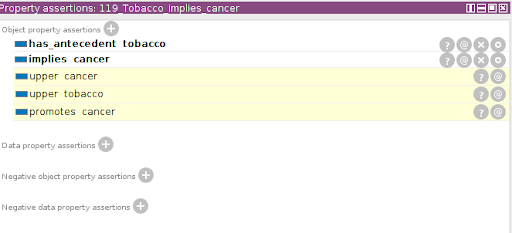
\includegraphics{promotes.png}
	\caption{Example of correct annotation for the \texttt{promotes} relation in Protege}
\label{fig:promotes_example}
\end{figure}

\subsubsection*{Suppresses}

Suppresses is the \textbf{opposite} of promotes. Everything valid for promotes
also applies to suppresses, but instead of causes you have
\texttt{does\_not\_cause} and instead of \texttt{implies} you have \texttt{contradicts}.

\paragraph{Declaration}

A declaration is simply a claim stating a domain concept either exists, should
be done or is good/bad. The claim \textit{mafia sells marijuana} is annotated by adding
the \texttt{has\_declaration} with the appropriate domain individual (as seen in Figure
\ref{fig:declaration_example}). 

\begin{figure}
	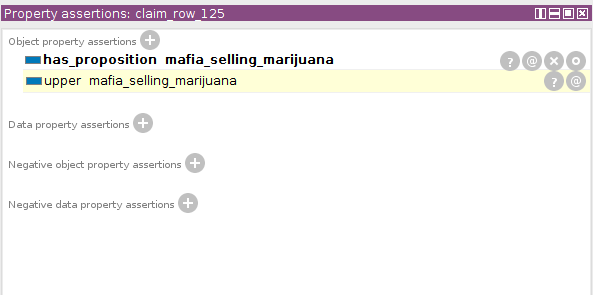
\includegraphics[scale=0.8]{has_declaration.png}
	\caption{Example of correct annotation for the \texttt{has\_declaration} relation in Protege}
\label{fig:declaration_example}
\end{figure}

\subsubsection*{Comparison}

Comparisons in debates arise when someone compares two domain individuals,
usually (but not always) by saying one is better according to some feature
(which is a domain individual). The comparison pattern is A is more than B by
C. The domain individual for more is annotated with
\texttt{comparison\_greater}, less is with \texttt{comparison\_less} and the
optional property of comparison is annotated with
\texttt{comparison\_property}. If there is no property, but an expression like
A is better than B is made, we don’t annotate \texttt{comparison\_property}.
The claim \textit{Alcohol is more influential on the mind than marijuana} is an
example annotated in the Figure~\ref{fig:comparison_example}.

\begin{figure}
	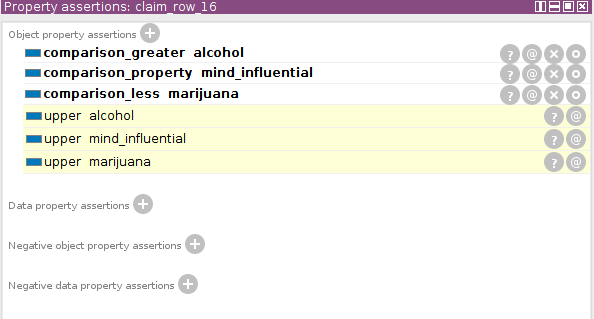
\includegraphics[scale=0.7]{comparison.png}
	\caption{Example of correct annotation for the \texttt{comparison} relation in Protege}
	\label{fig:comparison_example}
\end{figure}

\subsubsection*{Step 2.3 Negation}

If you think you need to negate the selected relation, for example in the
sentence: \textit{Marijuana legalization does not promote crime} the author explicitly
states that one domain individual \textbf{does not promote} another. As not promoting \textbf{is
not always} the same as suppresses, we allow you to add negation to any
relation to reflect that. To add negation, simply select ``Negative object
property assertions'' instead of ``Object property assertions'' along with your
relation. Example on the Figure \ref{fig:negation_example}. Be \underline{very careful}
when opting for negation, especially with double negation.

\begin{figure}
	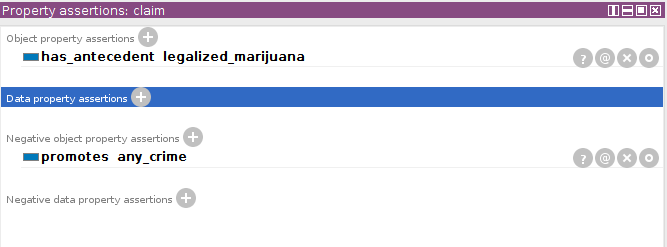
\includegraphics[scale=0.7]{negation.png}
	\caption{Example of correct annotation for negation in Protege}
	\label{fig:negation_example}
\end{figure}

\subsubsection*{Step 3 Selecting type}

We recognize that claims are made in a certain type (way which they were
expressed with) and discern between:

\begin{itemize}
\item \textbf{Facts}:  believes/argues/thinks that claim C is true (example:
	\textit{Marijuana is legal})
\item \textbf{Policies}: A believes/argues/thinks C should be true in the
	future or should remain true  (example: \textit{Marijuana should be legal}) 
\item \textbf{Value judgement}: A believes/argues/thinks C is morally/ethically
	right or wrong
	\begin{itemize}
	\item Judging of good (example: \textit{Marijuana is great})
	\item Judging of bad (example: \textit{Marijuana sucks})
	\end{itemize}
\end{itemize}
After recognizing the type, we need to add a property of \texttt{has\_type} which
can be one of \texttt{fact, policy, good\_value, bad\_value}. 

\subsubsection*{Opinion holder}

If the author mentions that his claim is made by someone else, we need to
annotate this information. For example, the following two claims are not made
by the same opinion holder:

\begin{enumerate}
\item Science says marijuana kills people
\item I think marijuana kills people
\end{enumerate}
For the first claim we need to add a property of \texttt{has\_opinion\_holder} to the
claim individual. The opinion holder can be any \textbf{domain individual}. In this
case, the opinion holder is science in claim 1). For claim 2), we don't need to
add a property \texttt{has\_opinion\_holder}, since the default opinion holder is the
author. 

\subsubsection*{Step 5 Claim annotation comments}

This is an optional step if you can't annotate the claim for some reason. You
need to annotate the claim individual with a comment if you can't get its
logical form. \textbf{All} claim individuals \textbf{should be annotated with logical form or
commented on}. Adding a comment is done by clicking '+' in the \texttt{Annotations} and
selecting \texttt{rdfs:comment} for a specific claim. If you're missing a domain
individual (see step 1), you can simply write \textit{missing domain individual X},
where X is the domain individual you deem required to get a logical form. 
Figure~\ref{fig:comment_example} shows 
a claim individual, upper pane shows the annotations part where
you can add your comment. 

\begin{figure}
	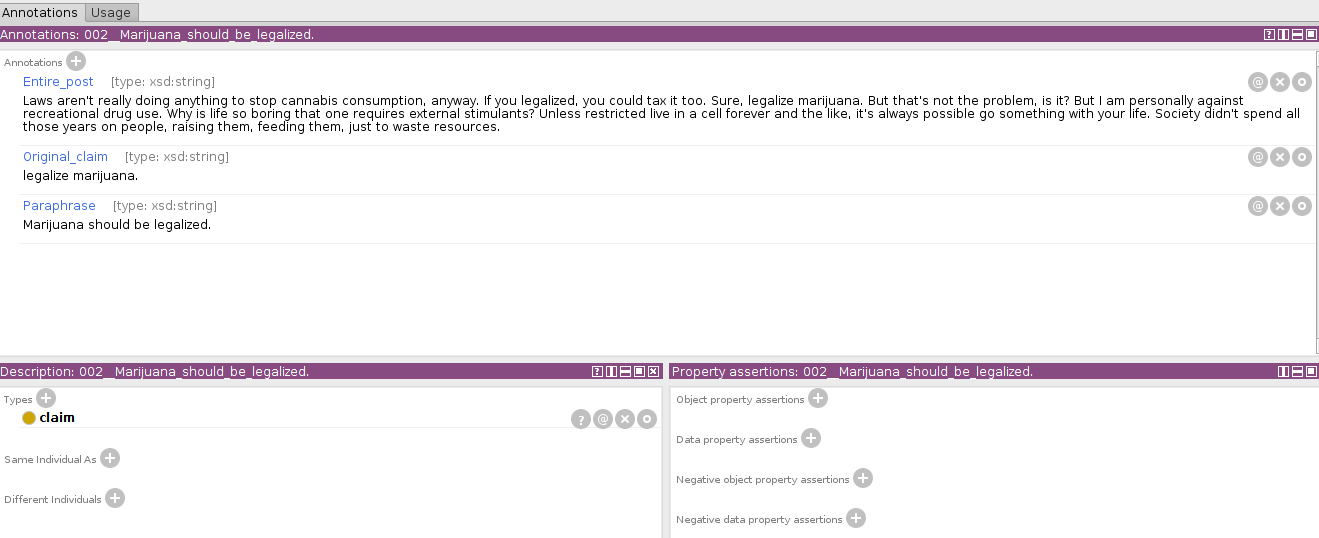
\includegraphics[scale=0.35]{comment.png}
	\caption{Example of correct annotation for adding a comment in Protege}
	\label{fig:comment_example}
\end{figure}

\subsection*{Annotation Examples}

\begin{mydef}
 \textit{Marijuana legalization will increase crime rate. }
\end{mydef}

\begin{enumerate}[label=\textbf{Step \arabic*.}, leftmargin=2cm, itemsep=0.5cm]
\item You need to see which domain individuals are mentioned in the claim.
\textit{Marijuana legalization} and \textit{crime rate} are candidate noun phrases which
might be a good place to start. 
\item You see there is a will increase verb and you consult with table in step
2.1. You can narrow down the choice between promotes, implies and
causes as one thing supports another (\textit{marijuana legalization}
and \textit{crime rate}).  
\item To get the type expressed you can work by elimination. Is there an
estimation if this is good or bad (if so, then value). Is there a
proposal of something that should be done? (if so, policy).
		Otherwise, it’s a factual information. 
\item There seems to be no mention of who is making the claim, so that should
	be the author. 
\end{enumerate}

\noindent Protege steps. 
\begin{enumerate}
\item Select the claim in Protege
\item Enter ``Object property assertions'' depending on the claim pattern identified 
\item Enter: \texttt{has\_antecedent} \texttt{legalized\_marijuana} (Step 1 \& 2)
\item Enter: \texttt{promotes any\_crime} (Step 1 \& 2)
\item Enter: \texttt{has\_type fact} (Step 3)
\end{enumerate}

\begin{mydef}
Growing marijuana does not make mafia stop selling marijuana.
\end{mydef}

\begin{enumerate}[label=\textbf{Step \arabic*.}, leftmargin=2cm, itemsep=0.5cm]
\item Here we start from domain individuals. Marijuana and mafia related domain
	individuals seem appropriate. Looking into possible options there is a
		domain individual of \texttt{marijuana\_farmer} which seems to be the
		closest to growing marijuana. For mafia, the most similar
		individual seems \texttt{mafia not selling marijuana}
\item  Focusing on the main verb phrase ``does not make'', we can notice the
	pattern A does not cause B, hence we pick \texttt{does\_not\_cause}. We omit the
		rest of the steps as they are similar to example 1. 
\end{enumerate}
Protege steps
\begin{enumerate}
\item Select the claim in Protege
\item Enter “Object property assertions”
\item Enter \texttt{has\_antecedent marijuana\_farmer} (Step 1\&2)
\item Enter \texttt{does\_not\_cause mafia\_not\_selling\_marijuana} (Step 1\&2)
\item Enter \texttt{has\_type fact} (Step 3)
\end{enumerate}
